\chapter {IMPLEMENTASI}
\par Bab ini membahas implementasi dari rancangan sistem yang ada pada bab 3. Bahasa pemrograman yang digunakan untuk implementasi aplikasi \textit{push notification}.

\section{Lingkungan Implementasi}
\par Lingkungan implementasi yang digunakan untuk mengembangkan tugas akhir ini memiliki spesifikasi perangkat keras dan lunak seperti ditampilkan pada tabel~\ref{tabel_spesifikasi_server}, tabel~\ref{tabel_spesifikasi_perangkat_android}, dan tabel~\ref{tabel_spesifikasi_perangkat_ios}.
\begin{longtable}{|p{2.5cm}|p{6.5cm}|}
    \hline
    \textbf{Jenis} & \textbf{Spesifikasi} & \hline
    CPU & AMD Ryzen 5 2500U & \hline
    Memory & 12 GB & \hline
    Sistem Operasi & Ubuntu 19.04 & \hline
    Kakas Bantu &
    \begin{enumerate}
        \item Intellij IDEA
        \item DataGrip
        \item Docker
    \end{enumerate} & \hline
    \caption{Spesifikasi Server}
    \label{tabel_spesifikasi_server}
\end{longtable}
\begin{longtable}{|p{2.5cm}|p{6.5cm}|}
    \hline
    \textbf{Jenis} & \textbf{Spesifikasi} & \hline
    CPU & Snapdragon 636 & \hline
    Memory & 3 GB & \hline
    Sistem Operasi & Android 9 (Pie) & \hline
    \caption{Spesifikasi Perangkat Android}
    \label{tabel_spesifikasi_perangkat_android}
\end{longtable}
\begin{longtable}{|p{2.5cm}|p{6.5cm}|}
    \hline
    \textbf{Jenis} & \textbf{Spesifikasi} & \hline
    CPU & Apple A10 Fusion & \hline
    Memory & 3 GB & \hline
    Sistem Operasi & iOS 12 & \hline
    \caption{Spesifikasi Perangkat iOS}
    \label{tabel_spesifikasi_perangkat_ios}
\end{longtable}

\section{Implementasi Basis Data}
\par Subbab ini membahas struktur tabel yang digunakan, meliputi tujuan pembuatan tabel, sumber kode yang digunakan untuk membuat tabel, dan gambar tabel yang telah dibuat.

\subsection{Implementasi Tabel User}
\par Tabel ini digunakan untuk menyimpan data pengguna.
\begin{lstlisting}[language=sql, firstnumber=1, caption=Implementasi Tabel User]
    create table user_account
    (
        user_id uniqueidentifier not null,
        name varchar(150) not null,
        nickname varchar(20),
        username varchar(255),
        password varchar(256) not null,
        email varchar(255),
        email_verified numeric(1) not null,
        scope varchar(4000),
        alternate_email varchar(255),
        alternate_email_verified numeric(1) not null,
        phone varchar(18),
        phone_verified numeric(1) not null,
        enabled numeric(1),
        picture varbinary(max),
        gender char,
        birthdate date,
        zoneinfo varchar(40),
        locale varchar(10),
        integra_id numeric(12),
        reg_id varchar(25),
        must_change_pwd numeric(1),
        sandbox numeric(1),
        locked datetime,
        suspended datetime,
        has_suspended numeric(1),
        group_id int not null,
        auth_method_id numeric(2),
        created_at datetime not null,
        update_at datetime not null,
        constraint PK_USER_ACCOUNT
            primary key (user_id),
        constraint FK_USER_ACC_AUTH_METH_AUTH_MET
            foreign key (auth_method_id) references auth_method,
        constraint FK_USER_ACC_USER_GROU_USER_GRO
            foreign key (group_id) references user_group
    )
\end{lstlisting}
\begin{figure}[H]
    \centering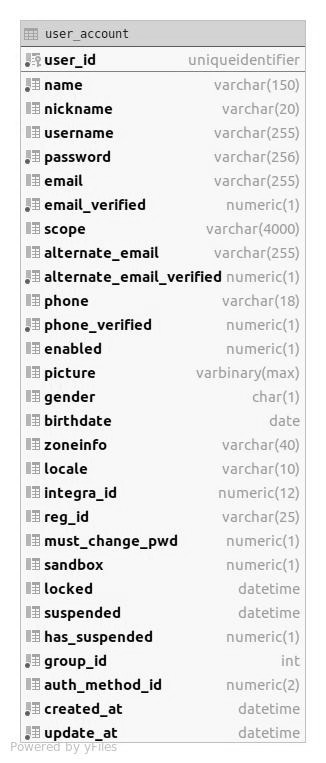
\includegraphics[width=0.5\textwidth]{bab4/figures/tabel_user_account.jpg}
    \caption{Tabel User (user\_account)}
    \label{tabel_user_account}
\end{figure}

\subsection{Implementasi Tabel Group}
\par Tabel ini digunakan untuk menyimpan data kelompok pengguna.
\begin{lstlisting}[language=sql, firstnumber=1, caption=Implementasi Tabel Group]
    create table pn_group
    (
        pn_group_id uniqueidentifier not null,
        name varchar(100),
        created_at datetime not null,
        update_at datetime not null,
        constraint PK_PN_GROUP
            primary key (pn_group_id)
    )
\end{lstlisting}
\begin{figure}[H]
    \centering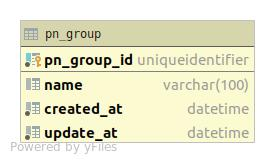
\includegraphics[width=0.5\textwidth]{bab4/figures/tabel_pn_group.jpg}
    \caption{Tabel Group (pn\_group)}
    \label{tabel_pn_group}
\end{figure}

\subsection{Implementasi Tabel Group Member}
\par Tabel ini digunakan untuk menyimpan data anggota kelompok pengguna.
\begin{lstlisting}[language=sql, firstnumber=1, caption=Implementasi Tabel Group Member]
    create table pn_group_member
    (
        pn_group_id uniqueidentifier not null,
        user_id uniqueidentifier not null,
        created_at datetime not null,
        update_at datetime not null,
        constraint PK_PN_GROUP_MEMBER
            primary key (pn_group_id, user_id),
        constraint FK_PN_GROUP_PN_GROUP__PN_GROUP
            foreign key (pn_group_id) references pn_group,
        constraint FK_PN_GROUP_USER_PN_G_USER_ACC
            foreign key (user_id) references user_account
    )
\end{lstlisting}
\begin{figure}[H]
    \centering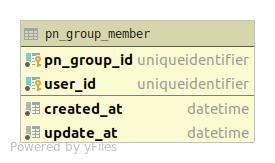
\includegraphics[width=0.5\textwidth]{bab4/figures/tabel_pn_group_member.jpg}
    \caption{Tabel Group Member (pn\_group\_member)}
    \label{tabel_pn_group_member}
\end{figure}

\subsection{Implementasi Tabel Client}
\par Tabel ini digunakan untuk menyimpan data client (aplikasi).
\begin{lstlisting}[language=sql, firstnumber=1, caption=Implementasi Tabel Client]
    create table oauth_client
    (
        client_id uniqueidentifier not null,
        client_name varchar(100) not null,
        client_description varchar(250),
        client_secret varchar(255),
        expires_at datetime,
        logo varchar(100),
        redirect_uri varchar(2000),
        post_logout_redirect_uris varchar(2048),
        frontchannel_logout_uri varchar(255),
        frontchannel_logout_session_required numeric(1),
        backchannel_logout_uri varchar(255),
        backchannel_logout_session_required numeric(1),
        base_uri varchar(255),
        api_base_uri varchar(255),
        app_type char,
        contact_name varchar(255),
        contact_email varchar(255),
        preauthorized numeric(1) not null,
        grant_types varchar(80),
        scope varchar(4000),
        sandbox numeric(1) not null,
        is_moderated numeric(1) not null,
        visible numeric(1) not null,
        category_id int,
        auth_type_id char,
        user_id uniqueidentifier,
        provider_id uniqueidentifier not null,
        created_at datetime not null,
        update_at datetime not null,
        constraint PK_OAUTH_CLIENT
            primary key (client_id),
        constraint FK_OAUTH_CL_AUTH_TYPE_AUTH_TYP
            foreign key (auth_type_id) references auth_type,
        constraint FK_OAUTH_CL_CLIENT_CL_CLIENT_C
            foreign key (category_id) references client_category,
        constraint FK_OAUTH_CL_PROVIDER__PROVIDER
            foreign key (provider_id) references provider,
        constraint FK_OAUTH_CL_USER_PIC_USER_ACC
            foreign key (user_id) references user_account
    )
\end{lstlisting}
\begin{figure}[H]
    \centering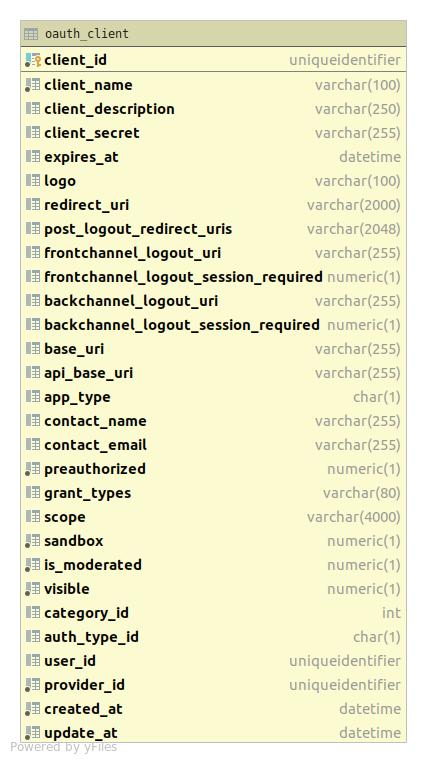
\includegraphics[width=0.5\textwidth]{bab4/figures/tabel_oauth_client.jpg}
    \caption{Tabel Client (oauth\_client)}
    \label{tabel_oauth_client}
\end{figure}

\subsection{Implementasi Tabel Certificate}
\par Tabel ini digunakan untuk menyimpan data sertifikat client untuk autentikasi ke layanan APNs dan FCM.
\begin{lstlisting}[language=sql, firstnumber=1, caption=Implementasi Tabel Certificate]
    create table pn_certificate
    (
        cert_id uniqueidentifier not null,
        client_id uniqueidentifier not null,
        bundle_id varchar(255),
        cert_key text,
        type char,
        password varchar(255),
        constraint PK_PN_CERTIFICATE
            primary key nonclustered (cert_id),
        constraint FK_PN_CERTI_OAUTH_CLI_OAUTH_CL
            foreign key (client_id) references oauth_client
    )
\end{lstlisting}
\begin{figure}[H]
    \centering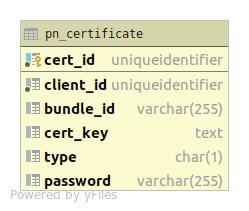
\includegraphics[width=0.5\textwidth]{bab4/figures/tabel_pn_certificate.jpg}
    \caption{Tabel Certificate (pn\_certificate)}
    \label{tabel_pn_certificate}
\end{figure}

\subsection{Implementasi Tabel Device}
\par Tabel ini digunakan untuk menyimpan data perangkat pengguna yang terdaftar di layanan APNs dan FCM.
\begin{lstlisting}[language=sql, firstnumber=1, caption=Implementasi Tabel Device]
    create table device_token
    (
        device_token_id uniqueidentifier not null,
        client_id uniqueidentifier not null,
        user_id uniqueidentifier not null,
        device_token varchar(255),
        device_type char,
        active numeric(1),
        reg_date datetime,
        invalidate_date datetime,
        constraint PK_DEVICE_TOKEN
            primary key (device_token_id),
        constraint FK_DEVICE_T_CLIENT_DE_OAUTH_CL
            foreign key (client_id) references oauth_client,
        constraint FK_DEVICE_T_USER_DEVI_USER_ACC
            foreign key (user_id) references user_account
    )
\end{lstlisting}
\begin{figure}[H]
    \centering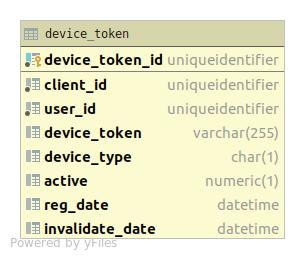
\includegraphics[width=0.5\textwidth]{bab4/figures/tabel_device_token.jpg}
    \caption{Tabel Device (device\_token)}
    \label{tabel_device_token}
\end{figure}

\subsection{Implementasi Tabel Batch}
\par Tabel ini digunakan untuk menyimpan data notifikasi yang akan dikirim ke beberapa pengguna atau kelompok.
\begin{lstlisting}[language=sql, firstnumber=1, caption=Implementasi Tabel Batch]
    create table pn_batch
    (
        pn_batch_id uniqueidentifier not null,
        title varchar(255),
        body varchar(255),
        image varchar(255),
        sound varchar(255),
        action varchar(255),
        additional_data text,
        delivery_date datetime,
        started_at datetime,
        finished_at datetime,
        is_allowed numeric(1) not null,
        user_sender_id uniqueidentifier,
        client_sender_id uniqueidentifier,
        client_dest_id uniqueidentifier,
        created_at datetime not null,
        update_at datetime not null,
        constraint PK_PN_BATCH
            primary key nonclustered (pn_batch_id),
        constraint FK_PN_BATCH_CLIENT_DE_OAUTH_CL
            foreign key (client_dest_id) references oauth_client,
        constraint FK_PN_BATCH_CLIENT_SE_OAUTH_CL
            foreign key (client_sender_id) references oauth_client,
        constraint FK_PN_BATCH_USER_SEND_USER_ACC
            foreign key (user_sender_id) references user_account
    )
\end{lstlisting}
\begin{figure}[H]
    \centering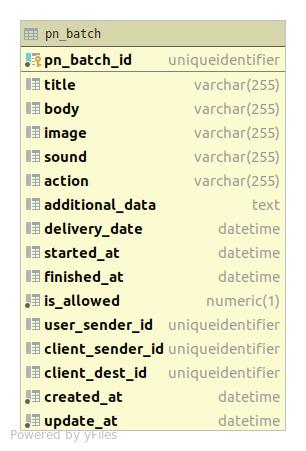
\includegraphics[width=0.5\textwidth]{bab4/figures/tabel_pn_batch.jpg}
    \caption{Tabel Batch (pn\_batch)}
    \label{tabel_pn_batch}
\end{figure}

\subsection{Implementasi Tabel Packet}
\par Tabel ini digunakan untuk menyimpan data notifikasi yang akan dikirim ke satu perangkat.
\begin{lstlisting}[language=sql, firstnumber=1, caption=Implementasi Tabel Packet]
    create table pn_packet
    (
        pn_packet_id uniqueidentifier not null,
        pn_batch_id uniqueidentifier not null,
        device_token_id uniqueidentifier,
        sent_at datetime,
        reason varchar(255),
        packet_status numeric(1) not null,
        created_at datetime not null,
        update_at datetime not null,
        constraint PK_PN_PACKET
            primary key (pn_packet_id),
        constraint FK_PN_PACKE_DEVICE_TO_DEVICE_T
            foreign key (device_token_id) references device_token,
        constraint FK_PN_PACKE_PN_BATCH__PN_BATCH
            foreign key (pn_batch_id) references pn_batch
    )
\end{lstlisting}
\begin{figure}[H]
    \centering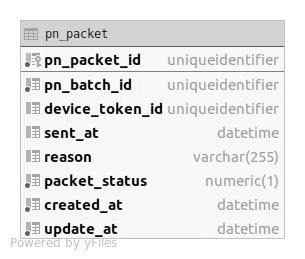
\includegraphics[width=0.5\textwidth]{bab4/figures/tabel_pn_packet.jpg}
    \caption{Tabel Packet (pn\_packet)}
    \label{tabel_pn_packet}
\end{figure}

\subsection{Implementasi Tabel User Destination}
\par Tabel ini digunakan untuk menyimpan data pengguna yang akan menerima notifikasi dari suatu batch.
\begin{lstlisting}[language=sql, firstnumber=1, caption=Implementasi Tabel User Destination]
    create table pn_user_destination
    (
        pn_batch_id uniqueidentifier not null,
        user_id uniqueidentifier not null,
        created_at datetime not null,
        update_at datetime not null,
        constraint PK_PN_USER_DESTINATION
            primary key (pn_batch_id, user_id),
        constraint FK_PN_USER__BATCH_USE_PN_BATCH
            foreign key (pn_batch_id) references pn_batch,
        constraint FK_PN_USER__USER_PN_D_USER_ACC
            foreign key (user_id) references user_account
    )
\end{lstlisting}
\begin{figure}[H]
    \centering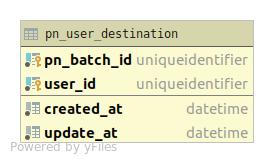
\includegraphics[width=0.5\textwidth]{bab4/figures/tabel_pn_user_destination.jpg}
    \caption{Tabel User Destination (pn\_user\_destination)}
    \label{tabel_pn_user_destination}
\end{figure}

\subsection{Implementasi Tabel Group Destination}
\par Tabel ini digunakan untuk menyimpan data kelompok yang akan menerima notifikasi dari suatu batch.
\begin{lstlisting}[language=sql, firstnumber=1, caption=Implementasi Tabel Group Destination]
    create table pn_group_destination
    (
        pn_batch_id uniqueidentifier not null,
        pn_group_id uniqueidentifier not null,
        created_at datetime not null,
        update_at datetime not null,
        constraint PK_PN_GROUP_DESTINATION
            primary key (pn_batch_id, pn_group_id),
        constraint FK_PN_GROUP_BATCH_GRO_PN_BATCH
            foreign key (pn_batch_id) references pn_batch,
        constraint FK_PN_GROUP_GROUP_PN__PN_GROUP
            foreign key (pn_group_id) references pn_group
    )
\end{lstlisting}
\begin{figure}[H]
    \centering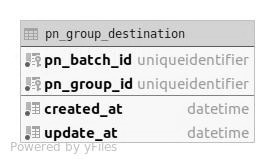
\includegraphics[width=0.5\textwidth]{bab4/figures/tabel_pn_group_destination.jpg}
    \caption{Tabel Group Destination (pn\_group\_destination)}
    \label{tabel_pn_group_destination}
\end{figure}

%TODO kopas kodingan
\section{Implementasi Proses dan Kasus Penggunaan}

\subsection{Implementasi Modul Scheduler}
\par Subbab ini membahas implementasi modul Scheduler berdasarkan kasus penggunaan aktor Scheduler.

\subsubsubsection{Implementasi Pembuatan Packet}
\par Proses pembuatan packet dilakukan secara berkala oleh modul Scheduler dengan interval waktu 1 menit.
Proses ini diawali dengan mencari data batch yang belum dan boleh diproses dari sistem basis data,
lalu mencari data device yang akan menerima notifikasi dari batch sistem basis data,
lalu untuk setiap device, data packet akan dibuat dan disimpan ke database.
Setelah packet berhasil dibuat, waktu pengiriman batch akan diperbarui menjadi waktu saat ini untuk menandai bahwa
batch tersebut telah selesai diproses.
Potongan kode yang digunakan untuk pembuatan packet dapat dilihat pada kode sumber [].
\subsubsection{Implementasi Pengiriman Packet ke Antrian}
\par Proses pengiriman packet ke antrian dilakukan secara berkala oleh modul Scheduler dengan interval waktu 1 menit
dan jeda awal 30 detik.
Proses ini diawali dengan mencari data packet yang sudah siap untuk dikirim (waktu pengiriman kurang dari waktu saat
ini) dari sistem basis data,
lalu packet tersebut akan diantrikan ke Kafka, dengan pembagian topik sesuai dengan jenis device penerima packet.
Potongan kode yang digunakan untuk pengiriman packet ke antrian dapat dilihat pada kode sumber [].

\subsection{Implementasi Modul Sender APN}
\par Subbab ini membahas implementasi modul Sender APN berdasarkan kasus penggunaan aktor Sender APN.

\subsubsection{Implementasi Pengiriman Packet ke APNs}
\par Proses pengiriman packet dilakukan secara berkala oleh Sender APN dengan cara menunggu Kafka untuk mengirimkan
data packet yang siap dikirim.
Proses ini diawali dengan Sender APN mendaftarkan diri di kafka sebagai consumer untuk topik ios,
lalu Kafka akan mengirimkan packet yang ada di antrian topik ios secara berkala ke Sender APN,
Setelah itu packet yang telah diterima akan dikirimkan oleh Sender APN ke layanan APNs.
Potongan kode yang digunakan untuk pengiriman packet ke APNs dapat dilihat pada kode sumber [].

\subsection{Implementasi Sender FCM}
\par Subbab ini membahas implementasi modul Sender FCM berdasarkan kasus penggunaan aktor Sender FCM.

\subsubsection{Implementasi Pengiriman Packet ke FCM}
\par Proses pengiriman packet dilakukan secara berkala oleh Sender FCM dengan cara menunggu Kafka untuk mengirimkan
data packet yang siap dikirim.
Proses ini diawali dengan Sender FCM mendaftarkan diri di kafka sebagai consumer untuk topik android dan web,
lalu Kafka akan mengirimkan packet yang ada di antrian topik android dan web secara berkala ke Sender FCM,
Setelah itu packet yang telah diterima dikirimkan oleh Sender FCM ke layanan FCM.
Potongan kode yang digunakan untuk pengiriman packet ke FCM dapat dilihat pada kode sumber [].
%\lstinputlisting[label=code:PacketConsumer, firstline=19, caption=Implementasi Kelas PacketConsumer, language=Java]
%{bab4/codes/sender-fcm/PacketConsumer.java}
